
\documentclass[11pt]{article}

% -------------------------------------------------
% Packages
% -------------------------------------------------
%\usepackage[margin=1in]{geometry}
\usepackage[
    top=1in,
    bottom=1in,
    left=.6in,
    right=.6in
]{geometry}
\usepackage{amsmath,amssymb,mathtools}
\usepackage{booktabs}
\usepackage{array}
\usepackage{enumitem}
\usepackage{listings}
\usepackage{xcolor}
\usepackage{hyperref}
\hypersetup{hidelinks}
\usepackage{float}
\usepackage{tikz}
\usepackage{pgfplots}
\usepackage{tabularx}
\pgfplotsset{compat=1.18}
\usepackage{parskip}

% -------------------------------------------------
% Simple notation
% -------------------------------------------------
\newcommand{\CFP}{C_{\mathrm{FP}}}
\newcommand{\CFN}{C_{\mathrm{FN}}}
\newcommand{\Risk}{\mathcal{R}}
\newcommand{\Prob}{\mathrm{P}}

\lstset{
  basicstyle=\ttfamily\small,
  frame=single,
  breaklines=true,
  columns=fullflexible,
  showstringspaces=false
}

% -------------------------------------------------
% Document
% -------------------------------------------------
\title{Cost Ratios, Probability Thresholds, Bayesian Decisions}
\author{DAEN 427/ISEN 427/ISEN 627 - Fall 2026}
\date{Alexander Abuabara}

\begin{document}

\maketitle

% \section{Purpose of This Note}

The previous class (i.e., week 3) introduced the Beta--Binomial Bayesian model and connected posterior uncertainty to decisions through a loss function. This note is a \emph{revision and clarification} of that material rather than a replacement for it. In particular, it focuses on the role of cost ratios, the distinction among several kinds of thresholds, and the transition from posterior uncertainty to an action. The central idea was:

\[
\boxed{
\text{probability model describes uncertainty}
\qquad
\text{loss model describes consequences}
}
\]

This note revises and clarifies that connection.

The main goal is to separate several quantities that can easily be confused:

\begin{enumerate}[label=\arabic*.]
    \item a \textbf{state or scientific threshold}, such as whether a true rate is above $0.50$;
    \item a \textbf{posterior or predictive probability} $q$;
    \item a \textbf{cost ratio}, such as $\CFN/\CFP$;
    \item an \textbf{action threshold} $\tau$ derived from the costs;
    \item a \textbf{classifier score threshold} when a model outputs probabilities or scores.
\end{enumerate}

The data and probability model determine what we believe.

The costs determine how strong that belief must be before taking an action.

\section{The Separation Principle}

Suppose there are two possible states:

\[
H=1
\qquad\text{and}\qquad
H=0,
\]

and two possible actions:

\[
a_+
=
\text{take the positive action},
\]

\[
a_-
=
\text{take the negative action}.
\]

Examples include:

\begin{center}
\begin{tabular}{lll}
\toprule
Context & Positive action $a_+$ & Negative action $a_-$ \\
\midrule
Fake news & Flag the article & Allow the article to pass \\
Chess player & He is goat & He is not so good \\
Inspection & Intervene & Do not intervene \\
Medical screening & Refer for follow-up & Do not refer \\
\bottomrule
\end{tabular}
\end{center}

Let

\[
q=\Prob(H=1\mid\text{information})
\]

be the relevant probability after incorporating the available information.

The probability model determines $q$.

The loss model determines what to do with $q$.

This is the key separation:

\[
\boxed{
\text{Prior + data}
\longrightarrow
q
}
\]

while

\[
\boxed{
\text{Consequences}
\longrightarrow
\text{action threshold}
}
\]

and finally

\[
\boxed{
q
\quad\text{is compared with}\quad
\tau.
}
\]

\section{The Loss Table}

Assume correct decisions have zero loss.

Let

\[
\CFP
\]

be the loss from taking the positive action when the state is actually negative, and let

\[
\CFN
\]

be the loss from taking the negative action when the state is actually positive.

The loss table is

\begin{center}
\begin{tabular}{c|cc}
\toprule
 & $H=1$ & $H=0$ \\
\midrule
Positive action $a_+$ & $0$ & $\CFP$ \\
Negative action $a_-$ & $\CFN$ & $0$ \\
\bottomrule
\end{tabular}
\end{center}

The labels ``false positive'' and ``false negative'' refer to the \emph{decision}, not to the Bayesian model itself.

\subsection{Posterior Expected Loss}

If the positive action is chosen, it is wrong only when $H=0$.

Since

\[
\Prob(H=0\mid\text{information})=1-q,
\]

the posterior expected loss is

\[
\Risk(a_+)
=
\CFP(1-q).
\]

If the negative action is chosen, it is wrong only when $H=1$.

Therefore,

\[
\Risk(a_-)
=
\CFN q.
\]

Choose the positive action when

\[
\Risk(a_+)<\Risk(a_-).
\]

Thus,

\[
\CFP(1-q)<\CFN q.
\]

Expanding,

\[
\CFP-\CFP q<\CFN q.
\]

Therefore,

\[
\CFP<q(\CFP+\CFN),
\]

so

\[
\boxed{
q>
\frac{\CFP}{\CFP+\CFN}.
}
\]

Define

\[
\boxed{
\tau
=
\frac{\CFP}{\CFP+\CFN}.
}
\]

Then the decision rule is simply

\[
\boxed{
\text{Take the positive action if } q>\tau.
}
\]

At equality, the two actions have the same posterior expected loss.

\section{The Cost Ratio Is Not the Threshold}

A common source of confusion is saying that the cost ratio \emph{is} the threshold.

It is not.

Suppose we define the false-negative to false-positive cost ratio as

\[
r
=
\frac{\CFN}{\CFP}.
\]

Then

\[
\tau
=
\frac{\CFP}{\CFP+\CFN}
=
\frac{1}{1+\CFN/\CFP}.
\]

Therefore,

\[
\boxed{
\tau=\frac{1}{1+r}.
}
\]

The cost ratio $r$ is transformed into a probability threshold.

For example:

\begin{center}
\begin{tabular}{ccc}
\toprule
$r=\CFN/\CFP$ & $\tau=1/(1+r)$ & Interpretation \\
\midrule
$1$ & $0.50$ & Equal error costs \\
$3$ & $0.25$ & False negatives cost three times as much \\
$9$ & $0.10$ & False negatives cost nine times as much \\
$1/3$ & $0.75$ & False positives cost three times as much \\
$1/9$ & $0.90$ & False positives cost nine times as much \\
\bottomrule
\end{tabular}
\end{center}

\begin{figure}[H]
\centering
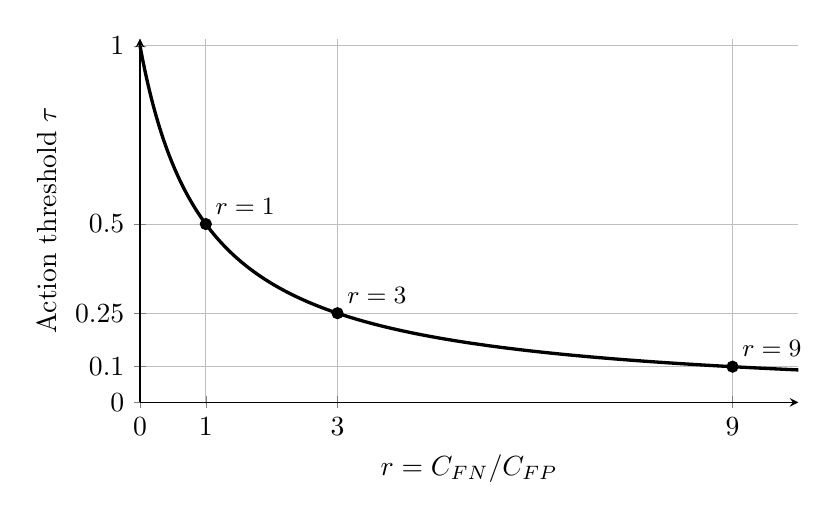
\begin{tikzpicture}
\begin{axis}[
    width=0.82\textwidth,
    height=6.2cm,
    xmin=0,
    xmax=10,
    ymin=0,
    ymax=1.02,
    axis lines=left,
    xlabel={$r=C_{FN}/C_{FP}$},
    ylabel={Action threshold $\tau$},
    xtick={0,1,3,9},
    ytick={0,0.1,0.25,0.5,1},
    grid=major,
    domain=0:10,
    samples=250,
    clip=false
]
\addplot[very thick,black] {1/(1+x)};
\addplot[only marks,mark=*,black] coordinates {
    (1,0.5)
    (3,0.25)
    (9,0.1)
};
\node[anchor=south west,font=\small] at (axis cs:1,0.5) {$r=1$};
\node[anchor=south west,font=\small] at (axis cs:3,0.25) {$r=3$};
\node[anchor=south west,font=\small] at (axis cs:9,0.1) {$r=9$};
\end{axis}
\end{tikzpicture}
\caption{The cost ratio $r=C_{FN}/C_{FP}$ is converted into the action threshold $\tau=1/(1+r)$. As false negatives become more costly relative to false positives, the probability required to justify the positive action decreases.}
\label{fig:cost-ratio-threshold}
\end{figure}

Figure~\ref{fig:cost-ratio-threshold} emphasizes that $r$ and $\tau$ are not the same quantity. The ratio $r$ is measured on a cost scale; $\tau$ is a probability between 0 and 1.

The direction is important:

\[
\CFN\uparrow
\quad\Longrightarrow\quad
\tau\downarrow.
\]

When missing a positive case becomes more expensive, less posterior probability is required before taking the positive action.

Similarly,

\[
\CFP\uparrow
\quad\Longrightarrow\quad
\tau\uparrow.
\]

When a false alarm becomes more expensive, stronger probability evidence is required before taking the positive action.

\subsection{Only the Relative Cost Matters}

If both costs are multiplied by the same positive constant $k$,

\[
\frac{k\CFP}{k\CFP+k\CFN}
=
\frac{\CFP}{\CFP+\CFN}.
\]

Therefore, under this simple loss structure, the action depends on the \emph{relative} costs, not their absolute scale.

For example,

\[
(\CFP,\CFN)=(1,3)
\]

and

\[
(\CFP,\CFN)=(100,300)
\]

produce the same threshold:

\[
\tau=0.25.
\]

\section{An Equivalent Odds Form}

Starting from

\[
\CFP(1-q)<\CFN q,
\]

divide both sides by $(1-q)\CFN$:

\[
\frac{q}{1-q}
>
\frac{\CFP}{\CFN}.
\]

Thus,

\[
\boxed{
\text{posterior odds}
>
\text{cost ratio in the opposite direction}.
}
\]

More explicitly,

\[
\boxed{
\frac{q}{1-q}
>
\frac{\CFP}{\CFN}.
}
\]

This form is often useful because it shows that the decision compares \emph{evidence expressed as odds} with \emph{relative consequences}.

\section{Three Different Thresholds Can Appear in One Problem}

The word ``threshold'' can refer to different quantities.

\subsection{State Threshold}

Suppose an unknown rate is denoted by $\pi$, and a state is defined as ``high'' when

\[
\pi>\pi_0.
\]

Then

\[
\pi_0
\]

is a \textbf{state threshold}.

It defines the event of interest.

\subsection{Posterior Probability of the State}

After observing data, compute

\[
q
=
\Prob(\pi>\pi_0\mid\text{data}).
\]

This is a probability about the state.

It is not itself a decision threshold.

\subsection{Action Threshold}

The loss model determines

\[
\tau
=
\frac{\CFP}{\CFP+\CFN}.
\]

The action is selected by comparing

\[
q
\quad\text{with}\quad
\tau.
\]

Therefore, the complete structure is

\[
\boxed{
\pi_0
\longrightarrow
q=\Prob(\pi>\pi_0\mid D)
\longrightarrow
q\ \text{vs.}\ \tau.
}
\]

\section{Why the Previous Example Can Be Confusing}

In the previous class, the Beta--Binomial example used a substantive threshold of

\[
\pi_0=0.50.
\]

The posterior calculation also produced

\[
q
=
\Prob(\pi>0.50\mid D)
=
0.50.
\]

Under equal error costs, the action threshold is also

\[
\tau=0.50.
\]

Thus, three different quantities happened to contain the number $0.50$:

\[
\boxed{
\pi_0=0.50,
\qquad
q=0.50,
\qquad
\tau=0.50.
}
\]

They represent different concepts.

Changing the cost ratio changes $\tau$, but it does not change the posterior distribution and therefore does not change $q$.

Changing the prior or the data can change $q$, but it does not automatically change the loss-based threshold $\tau$.

This distinction is central to Bayesian decision analysis.

\section{Revisiting the Fake-News Example}

We now use the fake-news data from the earlier Bayes' Rule class to make the cost-ratio idea concrete.

Define

\[
H=1
\quad\Longleftrightarrow\quad
\text{the article is fake}.
\]

The data contain

\[
60\text{ fake articles}
\]

and

\[
90\text{ real articles}.
\]

Thus the unconditional probability of fake news in the sample is

\[
\Prob(\text{Fake})
=
\frac{60}{150}
=
0.40.
\]

The headline evidence was whether the title contains an exclamation point.

The observed counts are

\begin{center}
\begin{tabular}{lrrr}
\toprule
Title contains ``!'' & Fake & Real & Total \\
\midrule
Yes & 16 & 2 & 18 \\
No & 44 & 88 & 132 \\
\midrule
Total & 60 & 90 & 150 \\
\bottomrule
\end{tabular}
\end{center}

\subsection{Empirical Conditional Probabilities}

For an article whose title contains an exclamation point,

\[
q_{!}
=
\Prob(\text{Fake}\mid !)
=
\frac{16}{18}
=
0.8889.
\]

For an article without an exclamation point,

\[
q_{\text{no }!}
=
\Prob(\text{Fake}\mid\text{no }!)
=
\frac{44}{132}
=
0.3333.
\]

These are probabilities of the positive state given the observed evidence.

They can therefore be compared directly with the cost-based action threshold.

\textbf{Examples:}

\begin{table}[ht]
\begin{tabularx}{\textwidth}{
    @{}
    >{\raggedright\arraybackslash}p{0.25\textwidth}
    >{\raggedright\arraybackslash}p{0.18\textwidth}
    >{\raggedright\arraybackslash}X
    @{}
}
\hline
\textbf{Situation} & \textbf{More costly} & \textbf{Reason} \\
\hline

Emergency or safety information
& False negative
& A fake article claiming that a contaminated food product is safe is classified as real, potentially leading to harmful decisions. \\

News archive or credibility-sensitive system
& False positive
& A legitimate investigative report is incorrectly labeled as fake and suppressed, potentially damaging credibility or limiting access to valid information. \\

Research benchmark or low-stakes news categorization
& Equal cost
& A real article classified as fake and a fake article classified as real are considered equally undesirable because neither error has substantially greater consequences. \\

\hline
\end{tabularx}

%%\caption{Examples of asymmetric and equal misclassification costs in fake news detection.}
\label{tab:fake_news_costs}
\end{table}

\section{Fake News Under Equal Costs}

Suppose

\[
\CFP=\CFN.
\]

Then

\[
r
=
\frac{\CFN}{\CFP}
=
1
\]

and

\[
\tau
=
\frac{1}{1+r}
=
0.50.
\]

For titles containing an exclamation point,

\[
0.8889>0.50,
\]

so the positive action is selected.

For titles without an exclamation point,

\[
0.3333<0.50,
\]

so the negative action is selected.

Thus, with equal costs, the exclamation point separates the two observed groups around the $0.50$ action threshold.
%%%%%%%%

\subsection{Equal-Cost Decisions and What the Data Say About the Threshold}

This clarifies two related but different questions:

\begin{enumerate}
    \item Why does an equal-cost decision rule use a threshold of $0.50$?
    \item If we look only at the observed fake-news data, what threshold is supported by the data?
\end{enumerate}

These questions should be kept separate. The value $0.50$ comes from the
\textbf{loss structure}, whereas the observed data determine which ranges of
thresholds produce different classifications.

\subsubsection*{Why Equal Costs Lead to a Threshold of 0.50}

Let

\[
q = P(\text{Fake} \mid \text{headline information}).
\]

There are two possible actions:

\[
a_{+} = \text{classify the article as fake},
\]

and

\[
a_{-} = \text{classify the article as real}.
\]

Let

\[
C_{FP}
\]

denote the cost of classifying a real article as fake, and let

\[
C_{FN}
\]

denote the cost of classifying a fake article as real.

The expected loss of classifying an article as fake is

\[
R(a_{+}) = C_{FP}(1-q),
\]

because this action is wrong only when the article is actually real.

The expected loss of classifying an article as real is

\[
R(a_{-}) = C_{FN}q,
\]

because this action is wrong only when the article is actually fake.

We choose the positive action when

\[
R(a_{+}) < R(a_{-}).
\]

Therefore,

\[
C_{FP}(1-q) < C_{FN}q.
\]

If false positives and false negatives have equal cost,

\[
C_{FP}=C_{FN}=C,
\]

then

\[
C(1-q)<Cq.
\]

Canceling $C$ gives

\[
1-q<q,
\]

so

\[
q>0.50.
\]

Thus, under equal costs,

\[
\boxed{\tau=0.50}.
\]

The important point is that this $0.50$ threshold is not estimated from the
fake-news data. It follows directly from the assumption that the two kinds of
classification errors have equal consequences.

\subsubsection*{Applying the 0.50 Decision Threshold to the Fake-News Data}

The fake-news data contain the following counts:

\begin{center}
\begin{tabular}{lrrr}
\toprule
Title contains ``!'' & Fake & Real & Total \\
\midrule
Yes & 16 & 2 & 18 \\
No  & 44 & 88 & 132 \\
\midrule
Total & 60 & 90 & 150 \\
\bottomrule
\end{tabular}
\end{center}

For articles containing an exclamation point,

\[
P(\text{Fake}\mid !)
=
\frac{16}{18}
\approx 0.8889.
\]

For articles without an exclamation point,

\[
P(\text{Fake}\mid \text{no }!)
=
\frac{44}{132}
=
0.3333.
\]

Under equal costs, compare each probability with the action threshold

\[
\tau=0.50.
\]

For titles containing an exclamation point,

\[
0.8889>0.50,
\]

so the lower expected-loss action is

\[
\boxed{\text{classify the article as fake}}.
\]

For titles without an exclamation point,

\[
0.3333<0.50,
\]

so the lower expected-loss action is

\[
\boxed{\text{classify the article as real}}.
\]

Therefore, the statement that the exclamation point ``separates'' the two
groups means only that the two estimated probabilities fall on opposite sides
of the $0.50$ decision boundary:

\[
\boxed{
P(\text{Fake}\mid\text{no }!)
<
0.50
<
P(\text{Fake}\mid !)
}.
\]

Numerically,

\[
\boxed{
0.3333 < 0.50 < 0.8889.
}
\]

This does \emph{not} mean that an exclamation point perfectly identifies fake
news. There are still two real articles with an exclamation point and 44 fake
articles without one. The exclamation point is useful evidence, but it is not
a perfect classifier.

\subsubsection*{What Threshold Is Suggested by the Data?}

Now consider a different question.

Suppose the classifier uses the rule

\[
\hat{Y}
=
\begin{cases}
\text{Fake}, & p\geq t,\\
\text{Real}, & p<t.
\end{cases}
\]

The data produce only two distinct estimated probabilities:

\[
p_{!}=0.8889
\]

and

\[
p_{\text{no }!}=0.3333.
\]

Therefore, changing the threshold $t$ can produce only three distinct
classification policies.

\begin{center}
\begin{tabular}{lll}
\toprule
Threshold range & Classification rule & Interpretation \\
\midrule
$t>0.8889$
&
Both groups classified real
&
No articles flagged
\\[4pt]

$0.3333<t\leq0.8889$
&
``!'' classified fake, no ``!'' classified real
&
Use headline evidence
\\[4pt]

$t\leq0.3333$
&
Both groups classified fake
&
All articles flagged
\\
\bottomrule
\end{tabular}
\end{center}

If we define ``best'' as minimizing the observed number of classification
errors, equivalent to using equal unit cost for every mistake, we can compare
the three policies.

\subsubsection*{Case 1: $t>0.8889$}

Every article is classified as real.

Therefore,

\[
FP=0,
\qquad
FN=60.
\]

The total number of errors is

\[
0+60=60.
\]

\subsubsection*{Case 2: $0.3333<t\leq0.8889$}

Articles with ``!'' are classified as fake, while articles without ``!'' are
classified as real.

The confusion-matrix counts are

\[
TP=16,
\qquad
FP=2,
\qquad
FN=44,
\qquad
TN=88.
\]

Thus,

\[
\text{Errors}
=
FP+FN
=
2+44
=
46.
\]

The empirical error rate is

\[
\frac{46}{150}
\approx
0.307,
\]

and the empirical accuracy is

\[
\frac{16+88}{150}
=
\frac{104}{150}
\approx
0.693.
\]

\subsubsection*{Case 3: $t\leq0.3333$}

Every article is classified as fake.

Therefore,

\[
FP=90,
\qquad
FN=0.
\]

The total number of errors is

\[
90.
\]

Comparing the three possibilities,

\[
60,\qquad 46,\qquad 90,
\]

the smallest number of errors is obtained when

\[
\boxed{
0.3333<t\leq0.8889.
}
\]

Thus, the observed data do \emph{not} identify one unique optimal threshold.

Instead, under empirical $0$--$1$ loss, they identify an entire optimal
threshold region:

\[
\boxed{
t\in(0.3333,\,0.8889].
}
\]

Every threshold inside this interval produces exactly the same predictions for
these data.

For example,

\[
t=0.40,\qquad
t=0.50,\qquad
t=0.60,\qquad
t=0.80
\]

all produce the same classification:

\[
\text{``!''}\rightarrow\text{Fake},
\qquad
\text{no ``!''}\rightarrow\text{Real}.
\]

Consequently, the data alone provide no reason to prefer $0.50$ over $0.60$ or
$0.80$ within this interval.

\subsubsection*{Why 0.50 Is Still a Natural Choice Under Equal Costs}

The threshold

\[
t=0.50
\]

lies inside the empirically optimal region,

\[
0.3333<0.50\leq0.8889.
\]

Therefore, it produces the minimum observed number of mistakes for this simple
classifier.

However, the specific value $0.50$ has an additional decision-theoretic
interpretation: it follows from equal false-positive and false-negative costs.

Thus, two different arguments lead to compatible conclusions:

\[
\boxed{
\text{Data: }
0.3333<t\leq0.8889
}
\]

and

\[
\boxed{
\text{Equal costs: }
\tau=0.50.
}
\]

Since

\[
0.50\in(0.3333,0.8889],
\]

the equal-cost threshold is consistent with the empirically optimal threshold
region.

\subsubsection*{}

The key distinction is

\[
\boxed{
\text{the data determine where the probability scores lie;}
}
\]

\[
\boxed{
\text{the loss function determines where the decision boundary should lie.}
}
\]

For the fake-news example, the data provide the two scores

\[
0.3333
\qquad\text{and}\qquad
0.8889.
\]

These scores divide the threshold axis into three decision regions.

The cost model then determines which threshold is appropriate.

Under equal costs,

\[
C_{FP}=C_{FN},
\]

the decision threshold is

\[
\boxed{\tau=0.50}.
\]

Because

\[
0.3333<0.50<0.8889,
\]

this threshold classifies articles with an exclamation point as fake and
articles without an exclamation point as real.

A useful summary is therefore

\[
\boxed{
\text{data}
\longrightarrow
\text{possible threshold regions},
}
\]

while

\[
\boxed{
\text{costs}
\longrightarrow
\text{decision threshold within those regions}.
}
\]
```


%%%%%%%%
\section{Fake News When False Negatives Are More Expensive}

Suppose a false negative costs three times as much as a false positive:

\[
\CFN=3\CFP.
\]

Then

\[
r=3
\]

and

\[
\tau
=
\frac{1}{1+3}
=
0.25.
\]

Now

\[
q_{!}=0.8889>0.25
\]

and

\[
q_{\text{no }!}=0.3333>0.25.
\]

Therefore, the same probability model leads to more positive actions because the loss model has changed.

The data did not change.

The conditional probabilities did not change.

Only the consequences changed.

\section{Fake News When False Positives Are More Expensive}

Suppose instead that a false positive costs three times as much as a false negative:

\[
\CFP=3\CFN.
\]

Then

\[
r
=
\frac{\CFN}{\CFP}
=
\frac{1}{3}
\]

and

\[
\tau
=
\frac{1}{1+1/3}
=
0.75.
\]

Now

\[
0.8889>0.75
\]

but

\[
0.3333<0.75.
\]

The decision rule becomes more conservative because the cost of a false alarm has increased.

\section{Finding the Cost-Ratio Boundary Directly}

Sometimes we know $q$ and want to ask:

\begin{quote}
How large must the false-negative cost be, relative to the false-positive cost, before the positive action becomes optimal?
\end{quote}

Starting from

\[
q>\frac{1}{1+r},
\]

solve for $r$:

\[
q(1+r)>1,
\]

\[
qr>1-q,
\]

so

\[
\boxed{
r>\frac{1-q}{q}.
}
\]

This formula directly converts a probability into a critical cost ratio.

\subsection{Article With an Exclamation Point}

For

\[
q_{!}
=
\frac{16}{18},
\]

the boundary is

\[
r
>
\frac{2/18}{16/18}
=
\frac{2}{16}
=
0.125.
\]

Thus,

\[
\boxed{
r>0.125
}
\]

is sufficient for the positive action for this group.

\subsection{Article Without an Exclamation Point}

For

\[
q_{\text{no }!}
=
\frac{44}{132},
\]

the boundary is

\[
r
>
\frac{88/132}{44/132}
=
\frac{88}{44}
=
2.
\]

Thus,

\[
\boxed{
r>2
}
\]

is required for the positive action for this group.

\subsection{Decision Regions}

Combining the two boundaries gives three regions:

\[
\boxed{
\begin{array}{ll}
r<0.125
&
\Rightarrow
\text{negative action for both groups},
\\[6pt]
0.125<r<2
&
\Rightarrow
\text{positive action only for the ``!'' group},
\\[6pt]
r>2
&
\Rightarrow
\text{positive action for both groups}.
\end{array}
}
\]

At the boundary values, one of the groups is exactly indifferent under the assumed loss function.

This is the clearest way to see how the \textbf{cost ratio} controls the decision.

\begin{figure}[H]
\centering
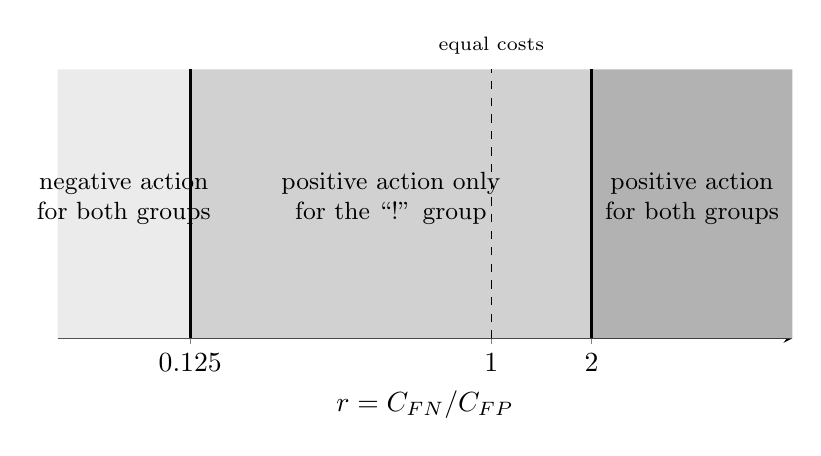
\begin{tikzpicture}
\begin{axis}[
    width=0.90\textwidth,
    height=5.0cm,
    xmode=log,
    log basis x=10,
    xmin=0.05,
    xmax=8,
    ymin=0,
    ymax=1,
    axis y line=none,
    axis x line=bottom,
    xlabel={$r=C_{FN}/C_{FP}$},
    xtick={0.125,1,2},
    xticklabels={$0.125$,$1$,$2$},
    ytick=\empty,
    clip=false
]
\addplot[draw=none,fill=black!8] coordinates {
    (0.05,0) (0.125,0) (0.125,1) (0.05,1)
} \closedcycle;
\addplot[draw=none,fill=black!18] coordinates {
    (0.125,0) (2,0) (2,1) (0.125,1)
} \closedcycle;
\addplot[draw=none,fill=black!30] coordinates {
    (2,0) (8,0) (8,1) (2,1)
} \closedcycle;
\draw[very thick] (axis cs:0.125,0) -- (axis cs:0.125,1);
\draw[very thick] (axis cs:2,0) -- (axis cs:2,1);
\draw[dashed] (axis cs:1,0) -- (axis cs:1,1);
\node[align=center,font=\small] at (axis cs:0.079,0.52) {negative action\\for both groups};
\node[align=center,font=\small] at (axis cs:0.50,0.52) {positive action only\\for the ``!'' group};
\node[align=center,font=\small] at (axis cs:4.0,0.52) {positive action\\for both groups};
\node[anchor=south,font=\scriptsize] at (axis cs:1,1.02) {equal costs};
\end{axis}
\end{tikzpicture}
\caption{Empirical decision regions for the fake-news example. The horizontal axis is logarithmic because $r$ is a positive ratio and the important changes are multiplicative. The decision changes at $r=0.125$ and $r=2$.}
\label{fig:fake-news-regions}
\end{figure}

Figure~\ref{fig:fake-news-regions} turns the algebra into a decision map. Moving from left to right means that false negatives become increasingly costly relative to false positives. The optimal action therefore becomes progressively more willing to flag an article as fake.

\section{The Same Result From Total Cost}

The same boundaries can be obtained by comparing total empirical cost.

If all articles are assigned the negative action:

\[
FP=0,
\qquad
FN=60,
\]

so

\[
C_{\text{all negative}}
=
60\CFN.
\]

If only articles with ``!'' receive the positive action:

\[
FP=2,
\qquad
FN=44,
\]

so

\[
C_{!}
=
2\CFP+44\CFN.
\]

If all articles receive the positive action:

\[
FP=90,
\qquad
FN=0,
\]

so

\[
C_{\text{all positive}}
=
90\CFP.
\]

Comparing these expressions produces the same critical ratios:

\[
r=0.125
\]

and

\[
r=2.
\]

This equivalence is useful:

\[
\boxed{
\text{case-by-case expected-loss rule}
\quad\Longleftrightarrow\quad
\text{aggregate cost minimization}
}
\]

when the probabilities and costs are defined consistently.

\section{The Earlier Fake-News Example with a Beta Prior}

The earlier fake-news example used the observed article counts to introduce Bayes' rule, including the empirical prior $P(\text{Fake})=0.40$ and the conditional evidence associated with exclamation points. It did \emph{not} specify separate Beta priors for the fake-news rates within the two headline groups.

The Beta model below is a new illustrative extension for this revision note. Its purpose is to connect the earlier fake-news example to the Beta--Binomial framework from the previous class. The choice

\[
\theta_g\sim\operatorname{Beta}(1,1)
\]

is not a prior supplied by the earlier presentation or inferred automatically from the data. It is an intentionally simple teaching prior. Different defensible prior information would produce different posterior parameters and, potentially, slightly different decision boundaries.

The empirical probabilities

\[
\frac{16}{18}
\qquad\text{and}\qquad
\frac{44}{132}
\]

treat the observed proportions as point estimates. Introducing a Beta prior lets us represent uncertainty about the underlying fake-news probability within each group.

\subsection{Titles With an Exclamation Point}

Let

\[
\theta_{!}
=
\Prob(\text{Fake}\mid !).
\]

We observe

\[
16\text{ fake}
\]

and

\[
2\text{ real}.
\]

Therefore,

\[
\theta_{!}\mid D
\sim
\operatorname{Beta}(1+16,1+2)
=
\operatorname{Beta}(17,3).
\]

\subsection{Titles Without an Exclamation Point}

Let

\[
\theta_{\text{no }!}
=
\Prob(\text{Fake}\mid\text{no }!).
\]

We observe

\[
44\text{ fake}
\]

and

\[
88\text{ real}.
\]

Thus,

\[
\theta_{\text{no }!}\mid D
\sim
\operatorname{Beta}(45,89).
\]

\section{Two Different Bayesian Questions}

The Beta posterior can support two different decision questions.

They should not be confused.

\subsection{Question A: Is the Next Article Fake?}

For the next article in group $g$, the posterior predictive probability of a fake article is

\[
q_g^{\mathrm{pred}}
=
\Prob(Y_{\mathrm{new}}=1\mid D,g).
\]

For a \emph{single} future binary outcome, the predictive model is most precisely described as \textbf{Beta--Bernoulli}: we integrate a Bernoulli outcome over the Beta posterior for $\theta_g$. Its success probability is the posterior mean,

\[
q_g^{\mathrm{pred}}
=
E(\theta_g\mid D).
\]

The term \textbf{Beta--Binomial posterior predictive} is appropriate when predicting the \emph{number} of fake articles among $m$ future articles. When $m=1$, that Beta--Binomial predictive calculation reduces to this one-trial Bernoulli result.

Thus,

\[
q_{!}^{\mathrm{pred}}
=
\frac{17}{17+3}
=
0.85,
\]

and

\[
q_{\text{no }!}^{\mathrm{pred}}
=
\frac{45}{45+89}
=
\frac{45}{134}
\approx
0.3358.
\]

These are the appropriate probabilities for a decision about the \emph{next individual article}.

\subsection{Question B: Is the Group's Underlying Fake Rate Above a Policy Level?}

Suppose instead that the question is whether the underlying group-level fake rate exceeds a threshold $\theta_0$.

Then the relevant probability is

\[
q_g^{\mathrm{rate}}
=
\Prob(\theta_g>\theta_0\mid D).
\]

For example, with

\[
\theta_0=0.50,
\]

we calculate

\[
q_{!}^{\mathrm{rate}}
=
\Prob(\theta_{!}>0.50\mid D)
=
1-F_{\operatorname{Beta}(17,3)}(0.50)
\approx
0.9996,
\]

while

\[
q_{\text{no }!}^{\mathrm{rate}}
=
\Prob(\theta_{\text{no }!}>0.50\mid D)
=
1-F_{\operatorname{Beta}(45,89)}(0.50)
\approx
0.000059.
\]

These answer a \emph{population-rate question}, not a next-article classification question.

The same Beta posterior supports both calculations, but the probability $q$ must match the actual decision problem.

\section{Posterior Predictive Cost-Ratio Boundaries for the Next Article}

Using the one-article Beta--Bernoulli posterior predictive probabilities, the positive action is selected when

\[
r>\frac{1-q}{q}.
\]

For the exclamation group,

\[
q=\frac{17}{20},
\]

so

\[
r
>
\frac{3/20}{17/20}
=
\frac{3}{17}
\approx
0.1765.
\]

For the no-exclamation group,

\[
q=\frac{45}{134},
\]

so

\[
r
>
\frac{89/134}{45/134}
=
\frac{89}{45}
\approx
1.9778.
\]

Therefore, with the illustrative $\operatorname{Beta}(1,1)$ prior:

\[
\boxed{
\begin{array}{ll}
r<0.1765
&
\Rightarrow
\text{negative action for both groups},
\\[6pt]
0.1765<r<1.9778
&
\Rightarrow
\text{positive action only for the ``!'' group},
\\[6pt]
r>1.9778
&
\Rightarrow
\text{positive action for both groups}.
\end{array}
}
\]

The boundaries differ slightly from the raw empirical values

\[
0.125
\quad\text{and}\quad
2
\]

because the Beta prior smooths the observed proportions.

\begin{center}
\begin{tabular}{lcc}
\toprule
Group & Empirical critical ratio & Beta(1,1) predictive critical ratio \\
\midrule
Title contains ``!'' & $0.1250$ & $0.1765$ \\
Title does not contain ``!'' & $2.0000$ & $1.9778$ \\
\bottomrule
\end{tabular}
\end{center}

The differences are modest here, but they reinforce the conceptual point: the probability model determines the probability used in the decision, while the cost ratio converts that probability into an action.

\section{A General Next-Case Decision Within the Beta--Binomial Framework}

The Beta--Binomial framework gives the Beta posterior for an unknown Bernoulli probability and a Beta--Binomial predictive distribution for counts in multiple future trials. For the special case of one next binary outcome, the predictive distribution is Bernoulli with probability equal to the posterior mean.

Suppose

\[
\theta\sim\operatorname{Beta}(\alpha,\beta)
\]

and we observe

\[
y
\]

positive outcomes in

\[
n
\]

trials.

Then

\[
\theta\mid D
\sim
\operatorname{Beta}
(\alpha+y,\beta+n-y).
\]

For the next binary outcome,

\[
q_{\mathrm{pred}}
=
\Prob(Y_{\mathrm{new}}=1\mid D)
=
\frac{\alpha+y}{\alpha+\beta+n}.
\]

The positive action is selected when

\[
q_{\mathrm{pred}}
>
\frac{1}{1+r}.
\]

Equivalently,

\[
\boxed{
r
>
\frac{\beta+n-y}{\alpha+y}.
}
\]

This formula directly links

\[
\boxed{
\text{prior information}
+
\text{observed counts}
+
\text{cost ratio}
}
\]

to the action for the next case.

\section{Classifier Probability Thresholds}

Suppose a classification model outputs a calibrated probability

\[
p_i
=
\Prob(Y_i=1\mid X_i).
\]

Under the same two-error loss table, the optimal action rule is

\[
\boxed{
p_i
>
\frac{\CFP}{\CFP+\CFN}.
}
\]

Thus, for a genuinely calibrated probability model,

\[
\boxed{
t^*
=
\tau
=
\frac{\CFP}{\CFP+\CFN}.
}
\]

However, if the model output is merely a score and is not calibrated as a probability, the numerical score threshold need not equal this expression.

In that case, one can evaluate candidate score thresholds empirically or calibrate the scores before applying the cost-based probability rule.

\section{Why ``Use 0.5'' Is Not a General Rule}

The value

\[
0.5
\]

is appropriate only under a particular combination of assumptions.

For the simple two-action loss table,

\[
\tau=0.5
\]

when

\[
\CFP=\CFN.
\]

If the costs are asymmetric, the threshold should move.

Therefore,

\[
\boxed{
0.5
\text{ is a special case, not a universal threshold.}
}
\]

The threshold is a decision quantity, not a property that automatically comes from the classification model.

\section{What the Data Determine and What the Costs Determine}

A useful decomposition is:

\[
\boxed{
\text{Prior + likelihood}
\longrightarrow
\text{posterior}
}
\]

\[
\boxed{
\text{Posterior}
\longrightarrow
q
}
\]

\[
\boxed{
\text{Costs}
\longrightarrow
\tau
}
\]

\[
\boxed{
q\ \text{vs.}\ \tau
\longrightarrow
\text{action}.
}
\]

The cost ratio does not change the posterior.

The prior does not directly specify the cost threshold.

The data do not determine how expensive a false positive or false negative should be.

Those are separate modeling choices.

\section{Sensitivity Analysis}

A decision is potentially fragile when

\[
q\approx\tau.
\]

Small changes in the prior, data, cost ratio, or model assumptions may then change the action.

Useful sensitivity checks include:

\begin{itemize}
    \item varying the Beta prior concentration while holding its mean fixed;
    \item varying the false-negative to false-positive cost ratio $r$;
    \item checking whether the posterior probability $q$ crosses the action threshold;
    \item examining whether a classifier's probabilities are calibrated;
    \item reconsidering assumptions such as conditional independence or representative sampling.
\end{itemize}

The important question is not only

\[
\text{``What action does the model imply?''}
\]

but also

\[
\text{``How much would our assumptions have to change before the action changes?''}
\]

\section{Common Sources of Confusion}

\begin{enumerate}[label=\arabic*.]
    \item \textbf{Confusing the state threshold with the action threshold.}

    A condition such as

    \[
    \pi>0.50
    \]

    defines the state. It does not imply that the posterior action threshold must also be $0.50$.

    \item \textbf{Calling the cost ratio the probability threshold.}

    If

    \[
    r=\frac{\CFN}{\CFP},
    \]

    then

    \[
    \tau=\frac{1}{1+r}.
    \]

    \item \textbf{Using the posterior mean when the decision concerns a tail probability.}

    If the question is whether

    \[
    \theta>\theta_0,
    \]

    the relevant quantity is

    \[
    \Prob(\theta>\theta_0\mid D),
    \]

    not simply

    \[
    E(\theta\mid D).
    \]

    \item \textbf{Using a tail probability when the decision concerns the next individual outcome.}

    For the next Bernoulli outcome, the relevant predictive probability is

    \[
    \Prob(Y_{\mathrm{new}}=1\mid D),
    \]

    which equals the posterior mean in the Beta--Bernoulli model.

    \item \textbf{Assuming the data determine the cost ratio.}

    Costs represent consequences or preferences. They must be specified from the decision context.

    \item \textbf{Assuming a default threshold of $0.5$ is always optimal.}

    It corresponds to equal false-positive and false-negative costs under the simple zero-loss-for-correct-decisions model.

    \item \textbf{Ignoring calibration.}

    The formula

    \[
    \tau=\frac{\CFP}{\CFP+\CFN}
    \]

    is a probability threshold. A generic uncalibrated model score is not automatically a probability.
\end{enumerate}

%\section{Compact R Workflow: Cost Ratio}
%
%The action threshold can be computed directly from the costs.
%
%\begin{lstlisting}[language=R]
%C_FP <- 1
%C_FN <- 3
%
%r <- C_FN / C_FP
%tau <- C_FP / (C_FP + C_FN)
%
%r
%tau
%# r   = 3
%# tau = 0.25
%\end{lstlisting}
%
%For the empirical fake-news probabilities:
%
%\begin{lstlisting}[language=R]
%q_bang <- 16 / 18
%q_no_bang <- 44 / 132
%
%tau <- 0.25
%
%q_bang > tau
%q_no_bang > tau
%\end{lstlisting}

%\section{Compact R Workflow: Beta--Binomial Fake-News Revision}
%
%Using a uniform $\operatorname{Beta}(1,1)$ prior:
%
%\begin{lstlisting}[language=R]
%alpha <- 1
%beta  <- 1
%
%# Title contains "!"
%y_bang <- 16
%n_bang <- 18
%
%a_bang <- alpha + y_bang
%b_bang <- beta + n_bang - y_bang
%
%q_pred_bang <- a_bang / (a_bang + b_bang)
%
%# Title does not contain "!"
%y_no <- 44
%n_no <- 132
%
%a_no <- alpha + y_no
%b_no <- beta + n_no - y_no
%
%q_pred_no <- a_no / (a_no + b_no)
%
%q_pred_bang
%q_pred_no
%\end{lstlisting}
%
%The cost-ratio boundary for each group is
%
%\begin{lstlisting}[language=R]
%rcrit_bang <- (1 - q_pred_bang) / q_pred_bang
%rcrit_no   <- (1 - q_pred_no) / q_pred_no
%
%rcrit_bang
%rcrit_no
%\end{lstlisting}
%
%For a group-level rate question such as
%
%\[
%\theta>0.50,
%\]
%
%use the Beta posterior tail probability:
%
%\begin{lstlisting}[language=R]
%q_rate_bang <- 1 - pbeta(
%  0.50,
%  shape1 = a_bang,
%  shape2 = b_bang
%)
%
%q_rate_no <- 1 - pbeta(
%  0.50,
%  shape1 = a_no,
%  shape2 = b_no
%)
%\end{lstlisting}

%\section{A Decision Checklist}
%
%Before making a cost-sensitive Bayesian decision, identify the following explicitly:
%
%\begin{enumerate}[label=\arabic*.]
%    \item What is the positive state?
%    \item What is the positive action?
%    \item What information defines the probability $q$?
%    \item Is $q$ a posterior state probability or a posterior predictive probability?
%    \item What exactly counts as a false positive?
%    \item What exactly counts as a false negative?
%    \item What are $\CFP$ and $\CFN$?
%    \item What is the ratio
%    \[
%    r=\CFN/\CFP?
%    \]
%    \item What action threshold follows?
%    \[
%    \tau=\frac{1}{1+r}.
%    \]
%    \item Is the final decision robust to reasonable changes in the prior, model, and costs?
%\end{enumerate}

\section{Summary}

The main conceptual revision is:

\[
\boxed{
\text{Probability and cost play different roles.}
}
\]

The probability model answers

\[
\boxed{
\text{How likely is the state that matters?}
}
\]

The loss model answers

\[
\boxed{
\text{How much evidence is enough to act?}
}
\]

For the two-error loss table,

\[
\Risk(a_+)=\CFP(1-q)
\]

and

\[
\Risk(a_-)=\CFN q.
\]

Therefore,

\[
\boxed{
q>
\frac{\CFP}{\CFP+\CFN}
}
\]

is the positive-action rule.

If

\[
r=\frac{\CFN}{\CFP},
\]

then

\[
\boxed{
\tau=\frac{1}{1+r}.
}
\]

Equivalently, for a known probability $q$, the positive action becomes optimal when

\[
\boxed{
r>\frac{1-q}{q}.
}
\]

For a Beta--Binomial model,

\[
\theta\mid D
\sim
\operatorname{Beta}(\alpha+y,\beta+n-y),
\]

and the next-case predictive probability is

\[
\boxed{
q_{\mathrm{pred}}
=
\frac{\alpha+y}{\alpha+\beta+n}.
}
\]

Combining this predictive probability with the cost ratio gives

\[
\boxed{
r>
\frac{\beta+n-y}{\alpha+y}.
}
\]

This last expression makes the full Bayesian decision structure explicit:

\[
\boxed{
\text{prior}
+
\text{data}
+
\text{consequences}
\longrightarrow
\text{decision}.
}
\]

\end{document}
